\documentclass[11pt]{article}

\usepackage{graphicx}

% Enable references to labels in the notes
\usepackage{xr-hyper}
\externaldocument{p328_notes}
\usepackage{hyperref}

% Sans fonts
\usepackage{sfmath}
\renewcommand{\familydefault}{\sfdefault}

\newcommand{\COURSE}{PHYS328W}
\newcommand{\LABNUM}{3}
\newcommand{\TITLE}{RC Filters}
\markright{\COURSE~Lab \LABNUM\ : \TITLE}

\setlength{\textwidth} {6.5 true in}
\setlength{\textheight}{9 true in}
\setlength{\hoffset}   {-0.75 true in}
\setlength{\voffset}   {-0.75 true in}
\setlength{\parindent} {12 pt}
\pagestyle{myheadings}

\begin{document}

\thispagestyle{empty}

\section*{\COURSE\ Lab \LABNUM\ : \TITLE}

This assignment relies on Section~\ref{sec:AC} of the notes.

\subsection*{Experiments}

\emph{The User Manual for your oscilloscope is available under Files
  on Canvas. The ``Operating basics'' section will orient you to the 
  display and control panel.}

\begin{figure}[h]
\centering
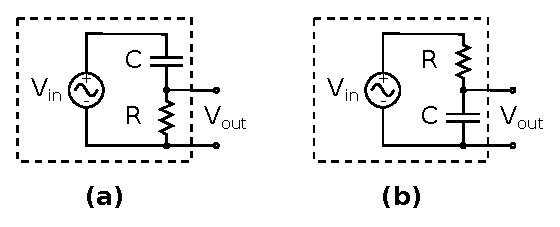
\includegraphics{rcvdividers.eps}
\caption{Series RC voltage dividers.}
\label{fig:rcvdividers}
\end{figure}

\begin{enumerate}
\item Check that your oscilloscope probes are compensated.

  \emph{See ``Manual probe compensation'' in the User Manual for
    your oscilloscope.}

\item Choose a resistor on the order of 1~k$\Omega$ and a capacitor on
  the order of 0.01~$\mu$F, and measure their values using the DMM.  

\item Construct either one of the circuits in
  Figure~\ref{fig:rcvdividers} on the breadboard using the function
  generator with a sinusoidal wave form and an amplitude of 1~V as
  your voltage source.

\item Set up the oscilloscope to display $V_{in}$ and $V_{out}$
  together, and use the oscilloscope and function generator to explore
  the frequency dependence of the gain $|V_{out}|/|V_{in}|$. 

  \emph{See ``Application examples'' $\rightarrow$ ``Taking simple
    measurements'' $\rightarrow$ ``Measuring two signals'' in the
    User Manual for your oscilloscope.}

\item Center both oscilloscope traces vertically, so that they share
  the same vertical zero point.
  \begin{itemize}
  \item On the Channel 1 and Channel 2 menus, switch the coupling to
    ground (GND), and center the traces vertically on the central grid
    line.
  \item Switch the coupling of both channels to \texttt{AC} to remove
    any DC offsets.
  \end{itemize}
  
\item Once you have a sense of the behavior of the circuit, measure
  $V_{in}$, $V_{out}$, and the phase angle (really, you'll be
  measuring $\Delta t$) at at least 10 frequencies that span the range
  over which the gain and phase angle are changing significantly.
  The phase angle $\phi$ is related to the time difference $\Delta t$
  between $V_{out}$ and $V_{in}$ via Equation~\ref{eq:deltatphi} in
  the notes. 

  \emph{To set up automated amplitude measurements, see ``Reference''
    $\rightarrow$ ``Measure'' in the User Manual for your
    oscilloscope, and for help measuring $\Delta t$ with the cursors,
    see ``Application examples'' $\rightarrow$ ``Taking Cursor
    Measurements.''}

\item Measure the 3~dB point of the circuit --- the point at
  which the transmitted \emph{power} is half of the
  incident power, which corresponds to a gain of $|V_{out}|/|V_{in}| =
  1/\sqrt{2}$.

\item Enter your data into a spreadsheet, and create voltage gain
  vs. frequency and phase angle vs. frequency plots.
\end{enumerate}

\subsection*{Calculations}

\begin{itemize}
\item In your log book, derive expressions for the gain, phase angle,
  and 3~dB point of the circuit, and calculate the 3~dB point. You may
  find Section~\ref{sec:acvdiv} of the notes helpful.

\item Add theoretical curves to the plots of measured voltage gain
  vs. frequency and phase angle vs. frequency in your spreadsheet.
\end{itemize}

\subsection*{Simulations}

\begin{enumerate}
\item Simulate your circuit using an \texttt{AC Sweep/Noise}
  simulation profile. Under \texttt{AC Sweep Type} choose
  \texttt{Logarithmic} with \texttt{Start Frequency:} 100,
  \texttt{End Frequency:} 1e6, and \texttt{Points/Decade:} 100. 

\item Place a voltage probe in the schematic to measure $V_{out}$.

\item Run the simulation. You should automatically see a plot of
  $V_{out}$ vs. frequency in the simulation results. Right-click on
  the trace and select \texttt{Copy to Clipboard}, and then paste the
  simulated data into your spreadsheet and add a simulated curve to
  your voltage gain vs. frequency plot.
  
\item Click on the 
\includegraphics{PSpiceAD_DefineMeasurement.png}
  button and set up a 3~dB point calculation. Use either
  \verb+Cutoff_Lowpass_3dB()+ or \verb+Cutoff_Highpass_3dB()+,
  depending on which circuit you chose. To show the
  measurement-results window, click on the
  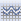
\includegraphics{PSpiceAD_ToggleMeasurement.png} button.
\end{enumerate}

\subsection*{Products}

Upload to Canvas ...

\begin{itemize}
\item A scan or image of your derivations of theoretical gain,
  phase angle, and 3-DB-point expressions. 

\item The PDF of a brief \LaTeX\ report in which you:
  \begin{itemize}
    \item Discuss the degree of agreement between your
      measurements, theoretical predictions, and simulation.

    \item Include as figures gain vs. frequency and phase angle
      vs. frequency plots. In the former, compare measurements, the
      theoretical curve, and the simulation. In the latter, compare
      measurements with the theoretical curve.

    \item Compare your measured, theoretical, and simulated 3~dB
      point results.

    \item Identify your circuit as either a high-pass or low-pass
      filter, and explain what that means.
  \end{itemize}
\end{itemize}

\end{document}
